\chapter{Introduction to Wireless Communication Systems} 
\section[Introduction]{\textbf{Introduction}}
Guglielmo Marconi invented the wireless radio system in 1895, and since then wireless communication has grown to become ubiquitous. As of 2018, there are 5.1 billion unique mobile phone users with this number expected to touch 5.8 billion between 2018-2025. \parencite{George2017}.
In all this time, the basic components of a wireless communication systems have remained the same as shown in Figure. 
\ref{fig:wireless block diagram}
\begin{figure}[htb]
\centering
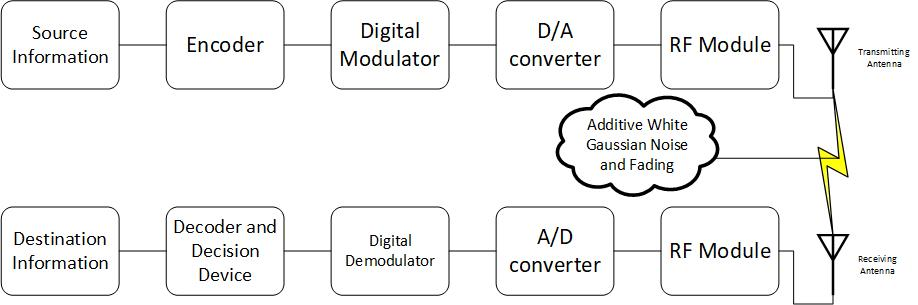
\includegraphics[scale=0.8]{Chapter 1/Figures/Wireless Communication System Block Diagram}
\caption{Wireless Digital Communication System}
\label{fig:wireless block diagram}
\end{figure}
 
In further chapters the discussion is on the various components of this system and the different techniques used in implementing them in \gls{matlab}. In this report the concern is only with the digital aspects of the system and not much attention is paid to the antenna parameters which can have a significant role to play in wireless systems. 


\section[Motivation]{\textbf{Motivation}}
There is an exponential increase in the number of new mobile users being added every year. Also, there are a host of services available for mobile users which demand high data rates. Video Teleconferencing, Real Time Video Streaming and other such services are some examples. These services coupled with the large number of people subscribing to such services means that there is a requirement for high capacity and high data rate systems.\\

At present the state of the art \acrshort{mimo} system is only being used in \gls{spatial diversity} mode which limits the capacity of the mobile system. Hence, it becomes attractive for telecom service providers to use the existing \acrshort{mimo} systems in \gls{spatial multiplexing} mode as well so that capacity is increased and at the same time maximum possible data rates are achieved for existing channel \acrshort{snr} conditions.  

\section[Problem statement]{\textbf{Problem statement}}
The problem statement which this report tries to address is the improvement of capacity and data rates in wireless communication systems. Using \acrshort{siso} systems, theoretically one can achieve high rates. However, there is a current discomfort with the design of these systems as there is a need to design complex equalizers, allocate large power budgets or have cost prohibitive modems all of which make  \acrshort{siso} systems unviable for communication.

\section[Objectives]{\textbf{Objectives}}
The objectives of the project is to initially build a \acrshort{siso} system which is used as a reference for further 2 antenna \acrshort{simo}, \acrshort{miso} systems. Finally a $2 \times 2$ \acrshort{mimo} systems is developed to examine ways to improve \acrshort{snr} for 2 antenna systems and capacity for high \acrshort{snr} regimes by using \acrshort{mcm}-\acrshort{mimo} systems.

\section{Literature Review}

\subsection{Multicarrier Systems}
The backbone of modern day \acrshort{4g} and \acrshort{5g} systems is the paradigm shift from single-channel systems to multi-carrier systems. This report is built upon the work of \textcite{Weinstein1971} where a low cost and easy to implement solution is offered with the help of an \acrshort{ifft} and \acrshort{fft} blocks which allows the system designer to use a single modulator rather than a block of modulators for each subchannel. This coupled with multiplexing capabilities of \acrshort{ofdm} as discussed by \textcite{Wu1995} form the foundation upon which our project is based.
 
\subsection{Modulation and Precoding Schemes}

\subsubsection{Modulation Schemes}
Coming to digital modulation schemes available at our disposal, the decision is made to use \acrshort{qam} as it is best suited for the purposes of this report. However, to achieve effective higher order \acrshort{qam} constellations this report follows in the work of \textcite{Bellili2015} to use a recursive algorithm that effectively maps symbols to higher order constellations in a computationally inexpensive manner. This method starts with the basic 4\acrshort{qam} and 8\acrshort{qam} constellations and dynamically creates higher order constellations without the need to save the points in memory.

\subsubsection{Precoding Schemes}
In certain cases, like $2 \times 1$ \acrshort{miso} systems where the choice is made to go for \gls{spatial diversity} scheme, this report includes some precoding measures as suggested by \textcite{Alamouti1998} so that the burden on the system is eased and overall system performance is improved. Apart from this this report also uses precoding schemes like inverse channel coders and singular value decomposers as suggested by \textcite{Klema1980} as huge improvements are noticed in speed by using these methods.

\subsection{Channel Modeling}
In terms of modeling the real world channel, one must consider various random processes to accurately define the channel. However, for the sake of simplicity this report models multipath systems as previously shown by \textcite{Hanlen2006} where more importance is placed on \gls{rayleigh fading} and ignore other effects like those of shadowing. Although, \gls{rayleigh fading} is a statistically simple model, it does a good job in showing the effects of fading on data signals while at the same time keeping complexity low. Channel estimation becomes an integral part of wireless systems as it directly correlates with the accuracy of our receiver and thereby our system performance.\\
Along with modeling fading, this report also take into consideration the aspects of noise that the channel adds to our data signal. Similarly as before, this report has chosen \acrshort{awgn} type of noise to represent an accurate but simplistic model. In the survey of literature it was noticed that most research scholars stick to a similar approach and this reports follows in the same footsteps.


\subsection{Transceiver Architecture and Channel Loading Methods}
\subsubsection{Transceiver Architecture}
In the design of the transmitter and receiver systems, this report relies upon standards set by the \acrshort{itu} as per their technical document \textcite{ITU2009}. This report builds upon the \gls{pilot signal} generation scheme provided here and suggest an alternative scheme with two $M \times N$ \acrshort{lfsr} banks to increase the dynamic range of the \acrshort{prbs} generator by observing the results of \textcite{Peinado2013}. This report also follows the same \textcite{ITU2009} standard in designing the transmitter and receiver systems to remain compliant with existing market service providers. The improvisation for the receiver comes in the form of \acrlong{svd} method as described by \textcite{Klema1980}. The claim is that this method enhances the system performance while reducing complexity making it commercially viable and attractive. 

\subsubsection{Channel Loading Methods}
Effective channel loading not only helps users with improving data rates but is also required for service providers to improve spectral efficiency. While studying the existing literature it was found that the method followed by \textcite{Chow1995} was effective but unsuitable as it is rate adaptive in nature. Therefore, this report draws inspiration from this tone loading algorithm to define a new fine gains algorithm to achieve an effective bit loading scheme. This loading scheme uses directly builds on the seminal work of \textcite{Shannon1948} and satisfies the requirements well while also being highly optimal.


\section{Brief Methodology of the project}
The basic methodology of this project is 
\begin{enumerate}
\item To develop an effective channel model for $2 \times 2$ \acrshort{mimo} links
\item To develop an efficient transmitter and receiver supporting \acrshort{mcm} and \acrshort{mimo} processing.
\end{enumerate}

To help achieve our objectives this report are follows the steps as stated below.

\begin{itemize}
\item A \acrshort{siso} system is developed for reference and this shows the performance of single channel systems to firmly establish the need for \acrshort{mcm}-\acrshort{mimo} systems.
\item Using this \acrshort{siso} system as a foundatio \acrshort{simo} and \acrshort{miso} systems are built which operate in diversity modes to elaborate how \acrshort{ber} can be improved for 2 antenna systems.
\item \gls{rayleigh fading} is introduced in the channel and modelling of \acrshort{los} path loss function is done with the help of Friis' formula.
\item The transmitter is assumed to be operating on a power budget of $1mW$.
\item Then a \acrshort{mimo} system is designed which is capable of operating in both diversity and multiplexing modes to finally observe the improvement in data rates and capacity over \acrshort{siso} systems.
\end{itemize}

\section{Organization of the report}

This report is organized as follows. 
\begin{itemize}
\item Chapter 2 discusses the fundamentals of \acrshort{mcm} and \acrshort{mimo} systems. The discussion is on the key technologies in \acrshort{mcm} and \acrshort{mimo} that enable it to be an effective solution for modern cellular systems. Along with this the chapter discusses some of the challenges faced in their implementation.
\item Chapter 3 informs the reader about the steps taken to design the communication system delving into the details of the design parameters and algorithms used. 
\item Chapter 4 shows the results obtained by performing simulations of our system on \gls{matlab}. Comparison of performance between existing systems and this system is shown and the effectiveness of this system is highlighted.
\item Chapter 5 is the final chapter where the report is concluded and the scope for future research is mentioned. This section also lists some additional features that can be added to the system to improve it. 
\end{itemize}

